\begin{landscape}


\subsection{Use Cases}

Starting from the requirements and generalizing scenarios we have
identified several use cases that represent basic functional units
carried out by TS. The following comprehensive UML diagram shows how
use cases are related one another and how actors interact with them;
each one is also provided with a table describing its main features.

\begin{figure}[H]
\begin{centering}
\includegraphics[bb=50bp 120bp 800bp 550bp,scale=0.75]{\string"specific-requirements/3.4-use-cases/image/use case\string".pdf}
\par\end{centering}

\protect\caption{UML Use Case Diagram}


\end{figure}


\end{landscape}

\clearpage{}


\subsubsection{Registration}

\begin{flushleft}
\begin{tabular}{c|>{\centering}p{10cm}}
\hline 
\emph{Name} & \raggedright{}Registration\tabularnewline
\hline 
\emph{Related goals} & \raggedright{}{[}G3{]}\tabularnewline
\hline 
\emph{Actors} & \raggedright{}Unregistered passenger\tabularnewline
\hline 
\emph{Entry condition} & \raggedright{}Nothing.\tabularnewline
\hline 
\emph{Flow of events} & \begin{enumerate}
\item \begin{raggedright}
Unregistered passenger opens the registration page on passenger's
application.
\par\end{raggedright}
\item \begin{raggedright}
Unregistered passengers fills the form with the required information
(firstname, lastname, email, username, password, address).
\par\end{raggedright}
\item \begin{raggedright}
Unregistered passenger agrees on terms and condition.
\par\end{raggedright}
\item \begin{raggedright}
Passenger's application submits the passenger's data to TS system.
\par\end{raggedright}
\item \begin{raggedright}
TS system checks their validity.
\par\end{raggedright}
\item \begin{raggedright}
TS system creates a new RegisteredPassenger with data provided by
unregistered passenger.
\par\end{raggedright}
\item \raggedright{}TS sends a confirmation e-mail to the user.\end{enumerate}
\tabularnewline
\hline 
\emph{Exit condition} & \raggedright{}The passenger information are lasting memorized in the
TS system.\tabularnewline
\hline 
\emph{Exceptions} & \begin{itemize}
\item \begin{raggedright}
If some information used to fill the form are invalid, the registration
process is interrupted and an error message is shown to the passenger.
The passenger can restart the procedure. 
\par\end{raggedright}
\item \raggedright{}If the procedure was interrupted before its termination
by external event (e.g. connection lost, system error, hardware failure)
the procedure is rolled back and no modifications are done in the
TS system.\end{itemize}
\tabularnewline
\hline 
\emph{Special requirements} & \raggedright{}Nothing.\tabularnewline
\hline 
\end{tabular}
\par\end{flushleft}

\clearpage{}

\begin{landscape}

\begin{figure}[H]
\begin{centering}
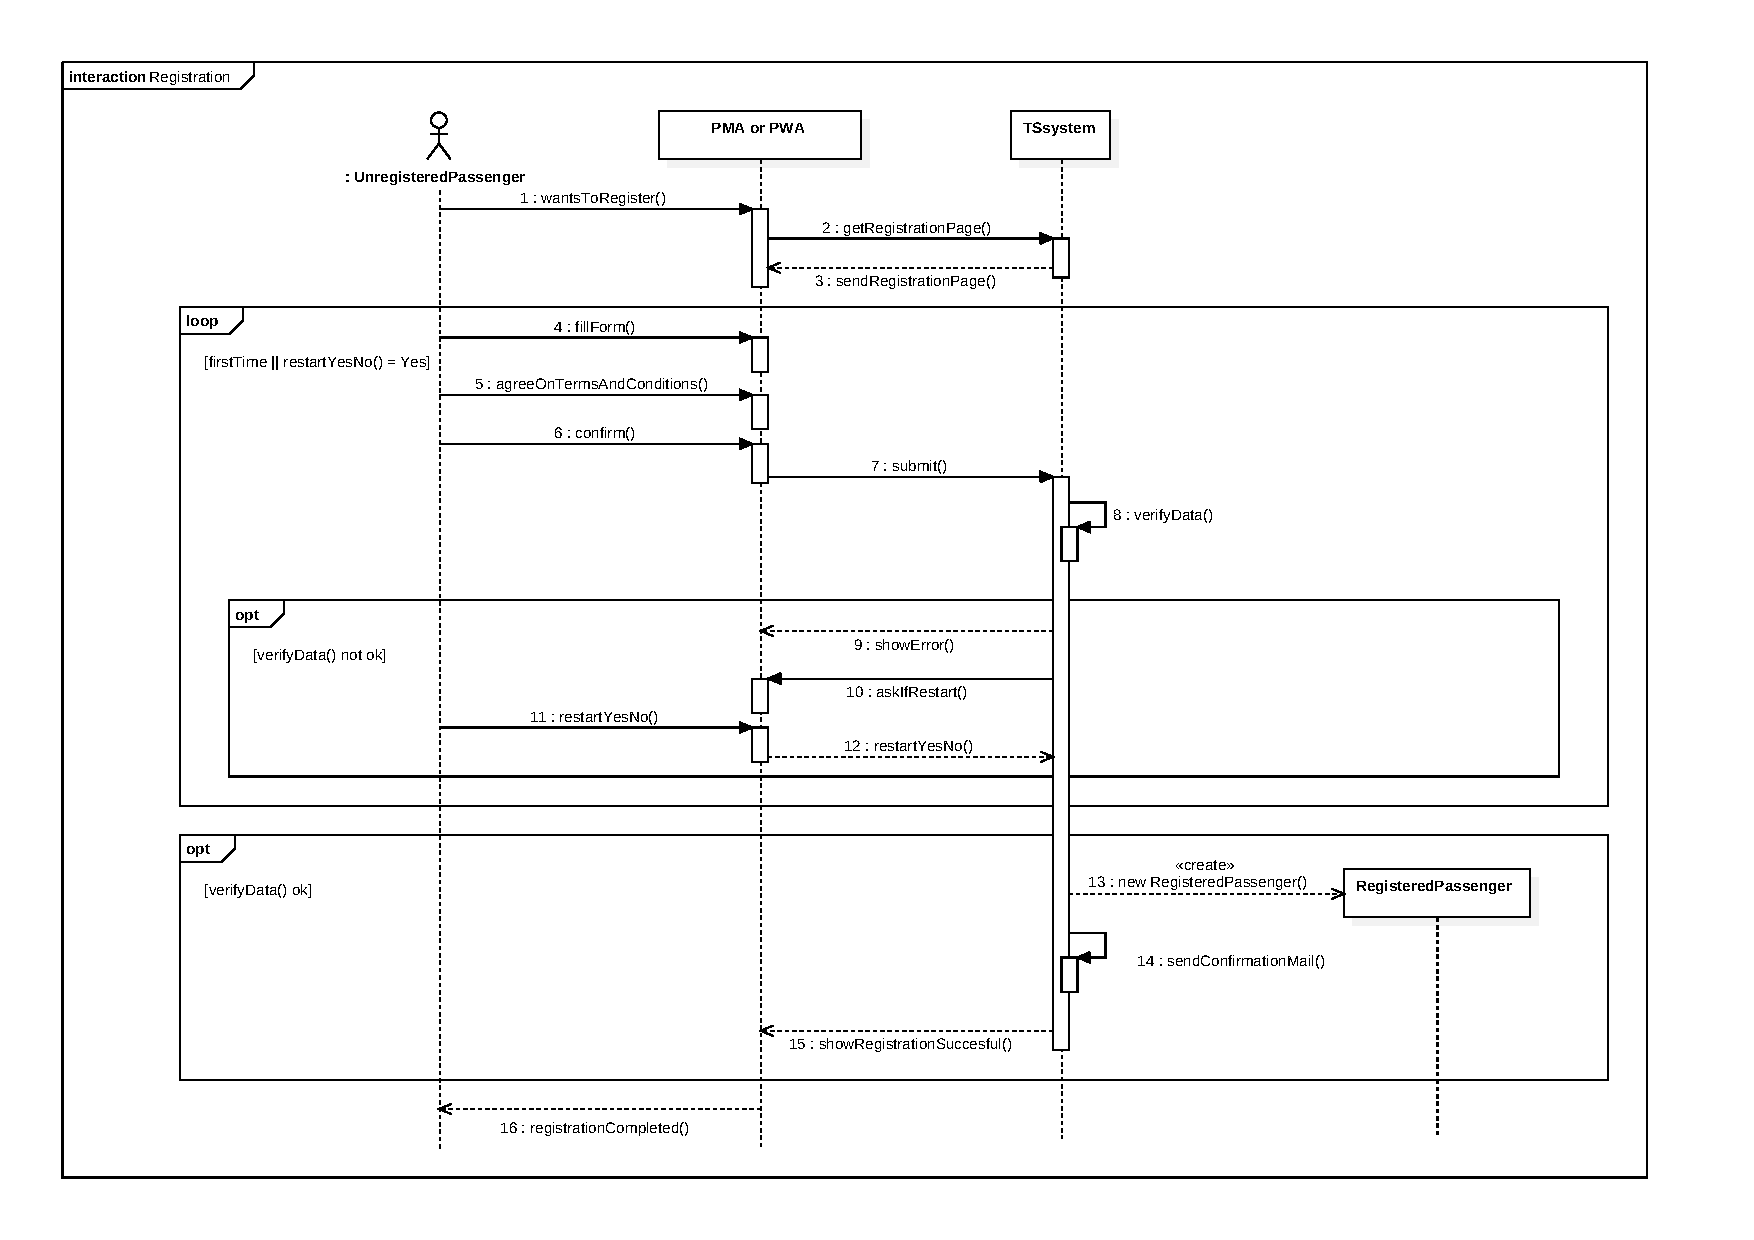
\includegraphics[bb=20bp 20bp 842bp 570bp,scale=0.7]{specific-requirements/3.4-use-cases/image/registration}
\par\end{centering}

\protect\caption{Registration - UML sequence diagram}


\end{figure}


\end{landscape}

\clearpage{}


\subsubsection{Request}

\begin{flushleft}
\begin{tabular}{c|>{\centering}p{10cm}}
\hline 
\emph{Name} & \raggedright{}Request\tabularnewline
\hline 
\emph{Related goals} & \raggedright{}{[}G1{]}\tabularnewline
\hline 
\emph{Actors} & \raggedright{}Passenger\tabularnewline
\hline 
\emph{Entry condition} & \raggedright{}Nothing.\tabularnewline
\hline 
\emph{Flow of events} & \begin{enumerate}
\item \begin{raggedright}
Passenger opens the request page on passengers' application.
\par\end{raggedright}
\item \begin{raggedright}
The passenger's application retrieves the localization asking to passenger
or using automatic geolocalization.
\par\end{raggedright}
\item \begin{raggedright}
Passenger inserts the number of passengers.
\par\end{raggedright}
\item \begin{raggedright}
Passanger accepts terms and conditions.
\par\end{raggedright}
\item \begin{raggedright}
Passenger's application sends data to QMA.
\par\end{raggedright}
\item \raggedright{}QMA creates a new request.\end{enumerate}
\tabularnewline
\hline 
\emph{Exit condition} & \raggedright{}A new request is created by QMA and ``Request evaluation''
is performed.\tabularnewline
\hline 
\emph{Exceptions} & \raggedright{}See ``Request without automatic geolocalization''
and ``Request with automatic geolocalization''.\tabularnewline
\hline 
\emph{Special requirement} & \raggedright{}Nothing.\tabularnewline
\hline 
\end{tabular}
\par\end{flushleft}


\subsubsection{Request without automatic geolocalization}

\begin{flushleft}
\begin{tabular}{c|>{\centering}p{10cm}}
\hline 
\emph{Name} & \raggedright{}Request without automatic geolocalization$\rightarrow$Request\tabularnewline
\hline 
\emph{Related goals} & \raggedright{}{[}G1{]}\tabularnewline
\hline 
\emph{Actors} & \raggedright{}Passenger\tabularnewline
\hline 
\emph{Entry condition} & \raggedright{}Device used to perform request that can't provide an
automatic geolocalization.\tabularnewline
\hline 
\emph{Flow of events} & \begin{enumerate}
\item \begin{raggedright}
Passenger opens the request page on passengers' application.
\par\end{raggedright}
\item \begin{raggedright}
Passenger specifies his/her address within passenger's application.
\par\end{raggedright}
\item \begin{raggedright}
Passenger inserts the number of passengers.
\par\end{raggedright}
\item \begin{raggedright}
Passanger accepts terms and conditions.
\par\end{raggedright}
\item \begin{raggedright}
Passenger's application sends data to QMA.
\par\end{raggedright}
\item \raggedright{}QMA creates a new request.\end{enumerate}
\tabularnewline
\hline 
\emph{Exit condition} & \raggedright{}A new request is created by QMA.\tabularnewline
\hline 
\emph{Exceptions} & \begin{itemize}
\item \raggedright{}If the address specified by passenger isn't found by
TS system (also considering very similar addresses) an error message
is sent and the user has to insert a new address.\end{itemize}
\tabularnewline
\hline 
\emph{Special requirement} & \raggedright{}Nothing.\tabularnewline
\hline 
\end{tabular}
\par\end{flushleft}

\clearpage{}


\subsubsection{Request with automatic geolocalization}

\begin{flushleft}
\begin{tabular}{c|>{\centering}p{10cm}}
\hline 
\emph{Name} & \raggedright{}Request with automatic localization $\rightarrow$Request\tabularnewline
\hline 
\emph{Related goals} & \raggedright{}{[}G1{]}\tabularnewline
\hline 
\emph{Actors} & \raggedright{}Passenger\tabularnewline
\hline 
\emph{Entry condition} & \raggedright{}Device used to perform request is able to provide a
automatic geolocalization.\tabularnewline
\hline 
\emph{Flow of events} & \begin{enumerate}
\item \begin{raggedright}
Passenger opens the request page on passengers' application.
\par\end{raggedright}
\item \begin{raggedright}
The passenger's application retrieves retives the localization using
automatic geolocalization.
\par\end{raggedright}
\item \begin{raggedright}
Passenger insterts the number of passengers.
\par\end{raggedright}
\item \begin{raggedright}
Passanger accepts terms and conditions.
\par\end{raggedright}
\item \begin{raggedright}
Passenger's application sends data to QMA.
\par\end{raggedright}
\item \raggedright{}QMA creates a new request.\end{enumerate}
\tabularnewline
\hline 
\emph{Exit condition} & \raggedright{}A new request is created by QMA.\tabularnewline
\hline 
\emph{Exceptions} & \begin{itemize}
\item \raggedright{}If the system fails to retrive automatic localization
or the information are invalid, an error message is shown and the
passenger that can insert manually the address (``Request without
automatic geolocalization'' is activated)\end{itemize}
\tabularnewline
\hline 
\emph{Special requirement} & \raggedright{}Nothing.\tabularnewline
\hline 
\end{tabular}
\par\end{flushleft}

\begin{landscape}

\begin{figure}[H]
\begin{centering}
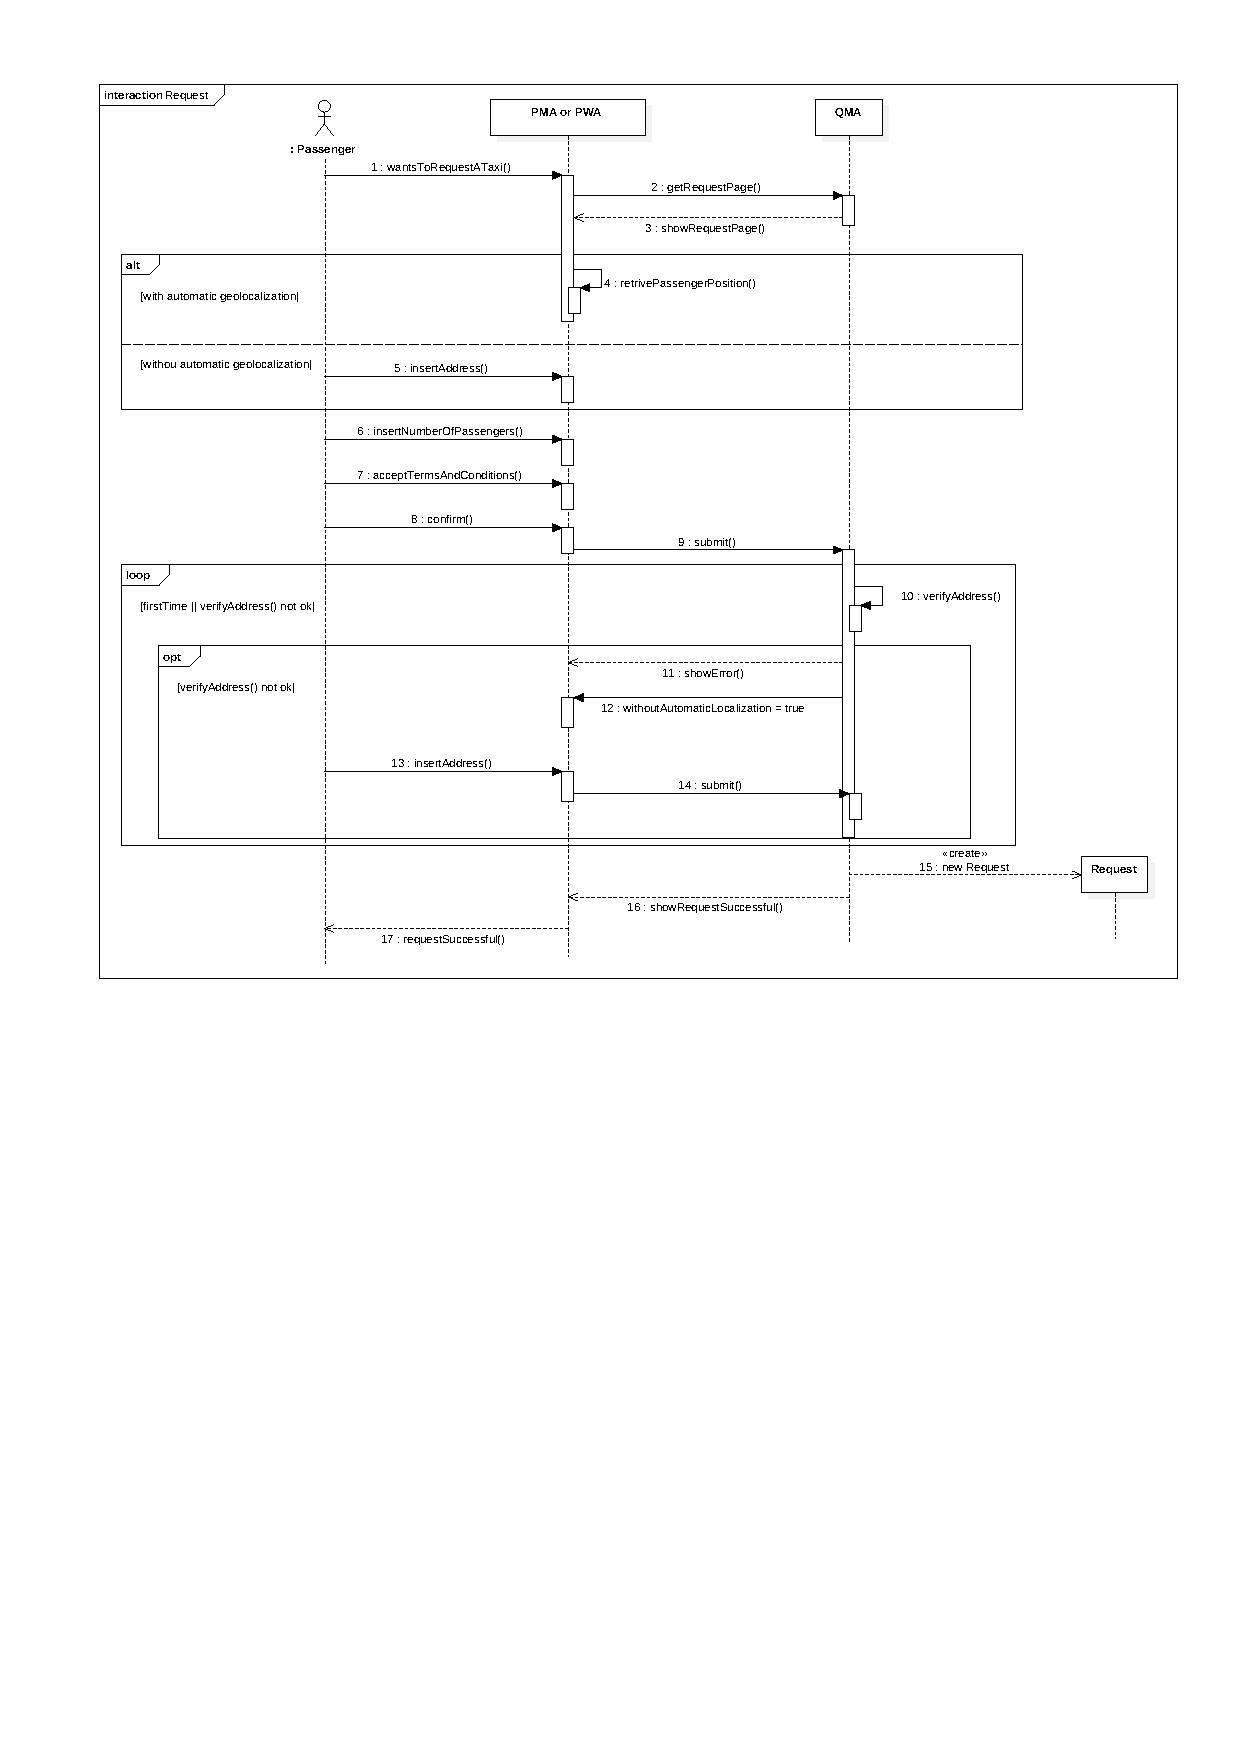
\includegraphics[bb=20bp 300bp 595bp 842bp,scale=0.7]{specific-requirements/3.4-use-cases/image/request}
\par\end{centering}

\protect\caption{Request - UML sequence diagram}
\end{figure}


\end{landscape}

\clearpage{}


\subsubsection{Login}

\begin{flushleft}
\begin{tabular}{c|>{\centering}p{10cm}}
\hline 
\emph{Name} & \raggedright{}Login\tabularnewline
\hline 
\emph{Actors} & \raggedright{}Registered passenger\tabularnewline
\hline 
\emph{Related goals} & \raggedright{}{[}G3{]}\tabularnewline
\hline 
\emph{Entry condition} & \raggedright{}The passenger is already registered to TS system.\tabularnewline
\hline 
\emph{Flow of events} & \begin{enumerate}
\item \begin{raggedright}
Passenger accesses to the login area.
\par\end{raggedright}
\item \begin{raggedright}
Passenger inserts credentials (username and password).
\par\end{raggedright}
\item \begin{raggedright}
The passenger's application sends the credentials to TS system.
\par\end{raggedright}
\item \begin{raggedright}
TS system checks for correctness of credentials.
\par\end{raggedright}
\item \raggedright{}TS system sends a confirmation to the passenger's application.\end{enumerate}
\tabularnewline
\hline 
\emph{Exit condition} & \raggedright{}Passenger can see personal area.\tabularnewline
\hline 
\emph{Exceptions} & \begin{itemize}
\item \raggedright{}If credentials are wrong, a message is shown to the
passenger and he is redirected to the login page.\end{itemize}
\tabularnewline
\hline 
\emph{Special requirement} & \raggedright{}Nothing.\tabularnewline
\hline 
\end{tabular}
\par\end{flushleft}

\clearpage{}

\begin{landscape}

\begin{figure}[H]
\begin{centering}
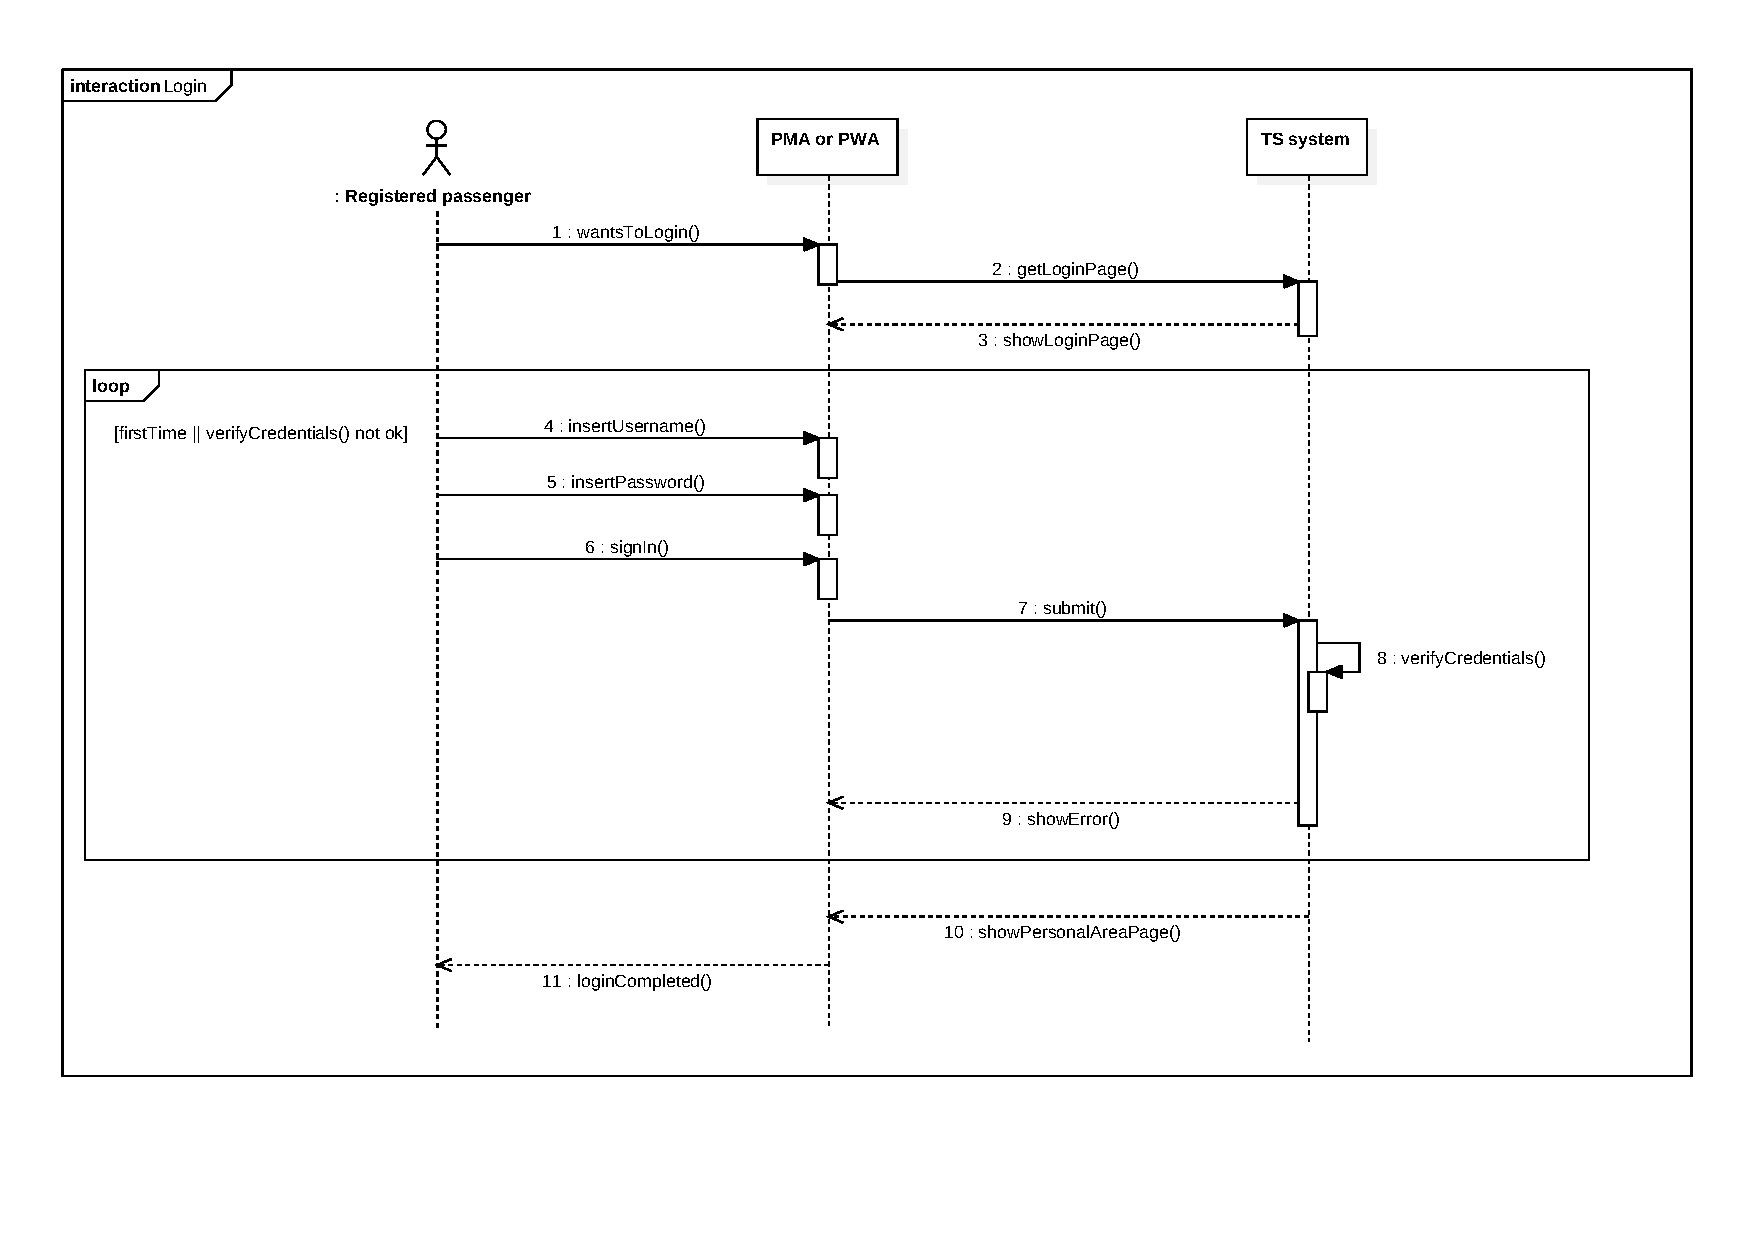
\includegraphics[bb=20bp 80bp 830bp 580bp,scale=0.75]{specific-requirements/3.4-use-cases/image/login}
\par\end{centering}

\protect\caption{Login - UML sequence diagram}
\end{figure}


\end{landscape}

\clearpage{}


\subsubsection{Reservation}

\begin{flushleft}
\begin{tabular}{c|>{\centering}p{10cm}}
\hline 
\emph{Name} & \raggedright{}Reservation\tabularnewline
\hline 
\emph{Related goals} & \raggedright{}{[}G4{]}\tabularnewline
\hline 
\emph{Actors} & \raggedright{}Registered passenger\tabularnewline
\hline 
\emph{Entry condition} & \raggedright{}Passenger is logged in.\tabularnewline
\hline 
\emph{Flow of events} & \begin{enumerate}
\item \begin{raggedright}
Passenger accesses to the reservation area.
\par\end{raggedright}
\item \begin{raggedright}
Passenger inserts the required data (address, date, time, number of
passengers).
\par\end{raggedright}
\item \begin{raggedright}
Passenger confirms the reservation.
\par\end{raggedright}
\item \begin{raggedright}
TS system whether data are valid. 
\par\end{raggedright}
\item \raggedright{}QMA creates a new reservation and the related request
is allocated.\end{enumerate}
\tabularnewline
\hline 
\emph{Exit condition} & \raggedright{}The reservation is added to the TS system.\tabularnewline
\hline 
\emph{Exceptions} & \begin{itemize}
\item \begin{raggedright}
If passenger does not confirm the operation is not performed.
\par\end{raggedright}
\item \begin{raggedright}
If the data are not valid (address, number of passengers) an error
message is shown to passenger and the operation is not performed.
Passenger can repeat the process.
\par\end{raggedright}
\item \raggedright{}If the date and time are such that the reservation is
not made at least two hour in advance an error message is shown to
user and the operation is not performed. Passenger can repeat the
process.\end{itemize}
\tabularnewline
\hline 
\emph{Special requirement} & \raggedright{}Nothing.\tabularnewline
\hline 
\end{tabular}
\par\end{flushleft}

\clearpage{}

\begin{landscape}

\begin{figure}[H]
\begin{centering}
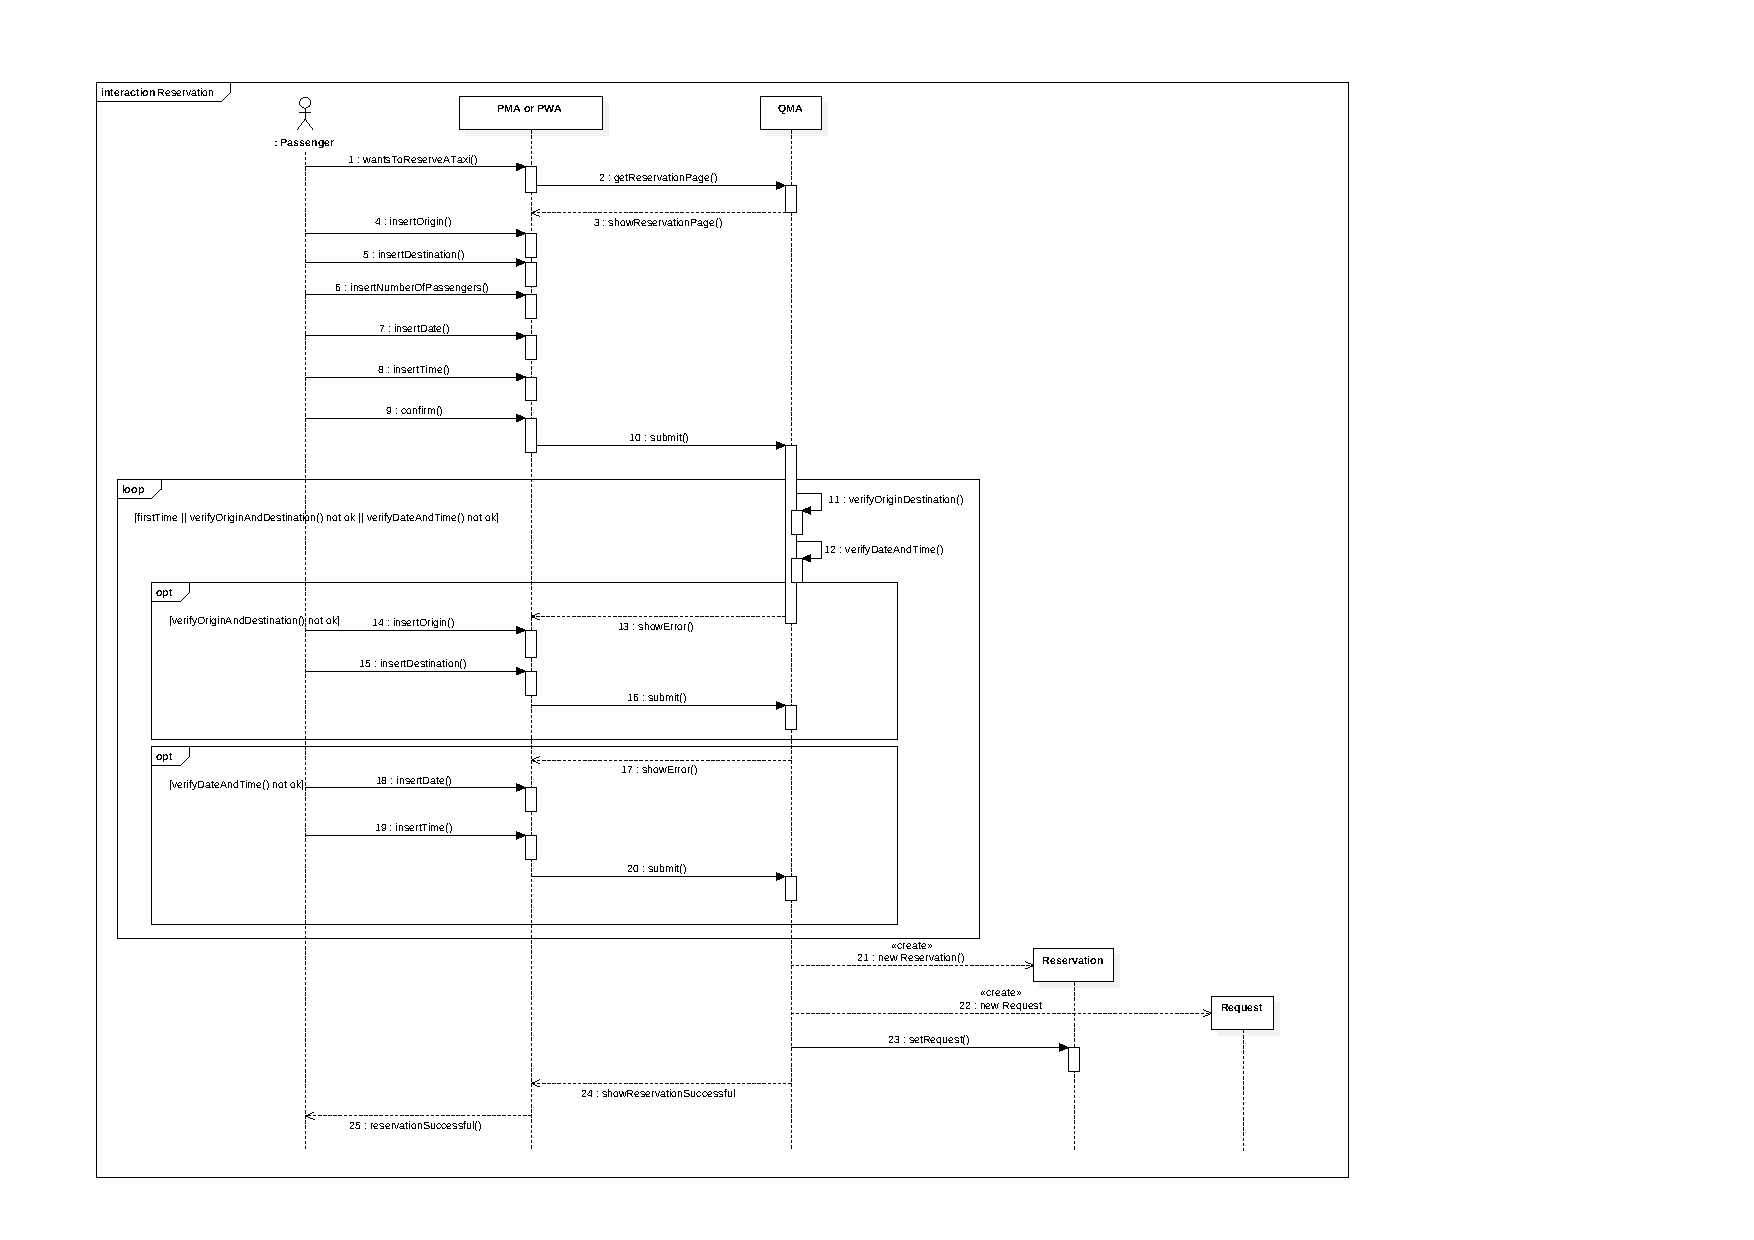
\includegraphics[bb=30bp 15bp 642bp 575bp,scale=0.7]{specific-requirements/3.4-use-cases/image/reservation}
\par\end{centering}

\protect\caption{Reservation - UML sequence diagram}
\end{figure}


\end{landscape}

\clearpage{}


\subsubsection{Cancel reservation}

\begin{flushleft}
\begin{tabular}{c|>{\centering}p{10cm}}
\hline 
\emph{Name } & \raggedright{}Cancel reservation\tabularnewline
\hline 
\emph{Related goals} & \raggedright{}{[}G5{]}\tabularnewline
\hline 
\emph{Actors} & \raggedright{}Registered passenger\tabularnewline
\hline 
\emph{Entry condition} & \raggedright{}Passenger has already forwarded a reservation and he/she
is logged in.\tabularnewline
\hline 
\emph{Flow of events} & \begin{enumerate}
\item \begin{raggedright}
Passenger accesses to previous reservations area.
\par\end{raggedright}
\item \begin{raggedright}
Passenger selects the reservation to be canceled.
\par\end{raggedright}
\item \begin{raggedright}
TS asks passenger for a confirmation.
\par\end{raggedright}
\item \begin{raggedright}
Passengers confirms the operation.
\par\end{raggedright}
\item \raggedright{}TS system removes the reservation and the associated
request.\end{enumerate}
\tabularnewline
\hline 
\emph{Exit condition} & \raggedright{}The reservation is delated by the TS system.\tabularnewline
\hline 
\emph{Exceptions} & \begin{itemize}
\item \raggedright{}If passenger does not confirm the operation is not performed.\end{itemize}
\tabularnewline
\hline 
\emph{Special requirement} & \raggedright{}Nothing.\tabularnewline
\hline 
\end{tabular}
\par\end{flushleft}

\clearpage{}

\begin{landscape}

\begin{figure}[H]
\begin{centering}
\includegraphics[bb=0bp 80bp 842bp 595bp,scale=0.7]{\string"specific-requirements/3.4-use-cases/image/cancel reserv\string".pdf}
\par\end{centering}

\protect\caption{Cancel reservation - UML sequence diagram}
\end{figure}


\end{landscape}

\clearpage{}


\subsubsection{Modify reservation}

\begin{flushleft}
\begin{tabular}{c|>{\raggedright}p{10cm}}
\hline 
\emph{Name } & \raggedright{}Modify reservation\tabularnewline
\hline 
\emph{Related goals} & \raggedright{}{[}G5{]}\tabularnewline
\hline 
\emph{Actors} & \raggedright{}Registered passenger\tabularnewline
\hline 
\emph{Entry condition} & \raggedright{}Passenger has already forwarded a reservation and he/she
is logged in.\tabularnewline
\hline 
\emph{Flow of events} & \begin{enumerate}
\item \begin{raggedright}
Passenger accesses to previous reservations area.
\par\end{raggedright}
\item \begin{raggedright}
Passenger selects the reservation to be modified.
\par\end{raggedright}
\item \begin{raggedright}
Passenger modifies data related to reservation (address, date time,
number of passengers).
\par\end{raggedright}
\item \begin{raggedright}
Passengers confirms the operation.
\par\end{raggedright}
\item The application sends the data to TS system.
\item \begin{raggedright}
TS system checks whether new data are valid.
\par\end{raggedright}
\item \raggedright{}QMA updates the reservation and the associated request.\end{enumerate}
\tabularnewline
\hline 
\emph{Exit condition} & \raggedright{}The modifications to the reservations are stored in
the the TS system.\tabularnewline
\hline 
\emph{Exceptions} & \begin{itemize}
\item \begin{raggedright}
If passenger does not confirm the operation is not performed.
\par\end{raggedright}
\item \begin{raggedright}
If the new data are not valid (address, date, time, number of passengers)
an error message is shown to passenger and the operation is not performed.
\par\end{raggedright}
\item \raggedright{}If the new date and time are such that the reservation
is not made at least two hour in advance an error message is shown
to user and the operation is not performed.\end{itemize}
\tabularnewline
\hline 
\emph{Special requirement} & \raggedright{}Nothing.\tabularnewline
\hline 
\end{tabular}
\par\end{flushleft}

\clearpage{}

\begin{figure}[H]
\begin{centering}
\includegraphics[scale=0.6]{\string"specific-requirements/3.4-use-cases/image/modify reserv\string".pdf}
\par\end{centering}

\protect\caption{Modify reservation - UML sequence diagram}
\end{figure}


\clearpage{}


\subsubsection{Queue management}

\begin{flushleft}
\begin{tabular}{c|>{\centering}p{10cm}}
\hline 
\emph{Name} & \raggedright{}Queue management\tabularnewline
\hline 
\emph{Related goals} & \raggedright{}{[}G8{]}\tabularnewline
\hline 
\emph{Actors} & \raggedright{}-\tabularnewline
\hline 
\emph{Entry condition} & \begin{itemize}
\item \begin{raggedright}
A new request is created or
\par\end{raggedright}
\item \begin{raggedright}
a taxi driver changes his state or
\par\end{raggedright}
\item \raggedright{}performed periodically.\end{itemize}
\tabularnewline
\hline 
\emph{Flow of events} & \begin{enumerate}
\item \begin{raggedright}
QMA retrives localization of each taxi and extracts the zone for each.
\par\end{raggedright}
\item \begin{raggedright}
QMA updates available taxi queue for each zone, possibly moving taxis
from a queue to an other (they are added at the end of the queue).
\par\end{raggedright}
\item \begin{raggedright}
QMA computes the taxis to be moved to one zone to another.
\par\end{raggedright}
\item \begin{raggedright}
QMA sends notification to those taxis.
\par\end{raggedright}
\item \raggedright{}QMA sets the state of those taxis to \emph{moving}.\end{enumerate}
\tabularnewline
\hline 
\emph{Exit condition} & \raggedright{}New distribution of taxis is stored in TS systems.\tabularnewline
\hline 
\emph{Exceptions} & \raggedright{}Nothing.\tabularnewline
\hline 
\emph{Special requirement} & \raggedright{}Nothing.\tabularnewline
\hline 
\end{tabular}
\par\end{flushleft}

\clearpage{}

\begin{figure}[H]
\begin{centering}
\includegraphics[scale=0.7]{\string"specific-requirements/3.4-use-cases/image/queue manag\string".pdf}
\par\end{centering}

\protect\caption{Queue Management - UML sequence diagram}
\end{figure}


\clearpage{}


\subsubsection{Visualize request info}

\begin{flushleft}
\begin{tabular}{c|>{\raggedright}p{10cm}}
\hline 
\emph{Name} & \raggedright{}Visualize request info\tabularnewline
\hline 
\emph{Related goals} & \raggedright{}{[}G2{]}\tabularnewline
\hline 
\emph{Actors} & \raggedright{}Passenger\tabularnewline
\hline 
\emph{Entry condition} & \raggedright{}Passenger has already made a request.\tabularnewline
\hline 
\emph{Flow of events} & \begin{enumerate}
\item \begin{raggedright}
Passenger's application asks QMA for waiting time and number of incoming
taxi.
\par\end{raggedright}
\item QMA calculates the requested information.
\item \begin{raggedright}
QMA sends those information to passenger's application.
\par\end{raggedright}
\item \raggedright{}Passenger's application display the information to the
passenger\end{enumerate}
\tabularnewline
\hline 
\emph{Exit condition} & \raggedright{}The requested information are shown to the passenger\tabularnewline
\hline 
\emph{Exceptions} & \raggedright{}Nothing.\tabularnewline
\hline 
\emph{Special requirement} & \raggedright{}Nothing.\tabularnewline
\hline 
\end{tabular}
\par\end{flushleft}

\clearpage{}

\begin{landscape}

\begin{figure}[H]
\begin{centering}
\includegraphics[scale=0.6]{\string"specific-requirements/3.4-use-cases/image/visualize req info\string".pdf}
\par\end{centering}

\protect\caption{Visualize request info - UML sequence diagram}
\end{figure}


\end{landscape}

\clearpage{}


\subsubsection{Request evaluation}

\begin{flushleft}
\begin{tabular}{c|>{\centering}p{10cm}}
\hline 
\emph{Name} & \raggedright{}Request evaluation\tabularnewline
\hline 
\emph{Related goals} & \raggedright{}{[}G6{]}\tabularnewline
\hline 
\emph{Actors} & \raggedright{}Taxi driver\tabularnewline
\hline 
\emph{Entry condition} & \raggedright{}A new request is created by QMA.\tabularnewline
\hline 
\emph{Flow of events} & \begin{enumerate}
\item \begin{raggedright}
QMA extracts the zone from which the request comes from.
\par\end{raggedright}
\item \begin{raggedright}
The request is forwarded to the first taxi (or taxis according to
the number of passengers) in the available taxis queue of the zone.
\par\end{raggedright}
\item \begin{raggedright}
Taxi driver sees on TMA informations related to the request (localization
and number of passengers).
\par\end{raggedright}
\item \raggedright{}See ``Request confirmation'' and ``Request rejection''.\end{enumerate}
\tabularnewline
\hline 
\emph{Exit condition} & \raggedright{}See ``Request confirmation'' and ``Request rejection''.\tabularnewline
\hline 
\emph{Exceptions} & \begin{itemize}
\item \begin{raggedright}
If the available taxi queue of the zone is empty, the operation is
repeated considering the queues of the adjacent zones.
\par\end{raggedright}
\item \begin{raggedright}
If no taxi is available at all, the request is put on hold until a
taxi becomes available.
\par\end{raggedright}
\item \raggedright{}If no answer in one minute it is interpreted as a rejection.\end{itemize}
\tabularnewline
\hline 
\emph{Special requirement} & \raggedright{}Nothing.\tabularnewline
\hline 
\end{tabular}
\par\end{flushleft}

\clearpage{}


\subsubsection{Request confirmation}

\begin{flushleft}
\begin{tabular}{c|>{\centering}p{10cm}}
\hline 
\emph{Name} & \raggedright{}Request confirmation$\rightarrow$Request evaluation\tabularnewline
\hline 
\emph{Related goals} & \raggedright{}{[}G6{]}\tabularnewline
\hline 
\emph{Actors} & \raggedright{}Taxi driver\tabularnewline
\hline 
\emph{Entry condition} & \raggedright{}A new request is created by QMA.\tabularnewline
\hline 
\emph{Flow of events} & \begin{enumerate}
\item \begin{raggedright}
QMA extracts the zone from which the request comes from.
\par\end{raggedright}
\item \begin{raggedright}
The request is forwarded to the first taxi in the available taxis
queue of the zone.
\par\end{raggedright}
\item \begin{raggedright}
Taxi driver sees on TMA informations related to the request (localization
and number of passengers).
\par\end{raggedright}
\item \begin{raggedright}
Taxi driver confirms the request.
\par\end{raggedright}
\item \begin{raggedright}
QMA sets taxi state as busy and removes it from the queue.
\par\end{raggedright}
\item \raggedright{}QMA computes the expected waiting time.\end{enumerate}
\tabularnewline
\hline 
\emph{Exit condition} & \raggedright{}A confirmed request is created in the system and ``Queue
management'' is performed.\tabularnewline
\hline 
\emph{Exceptions} & \begin{itemize}
\item \raggedright{}If waiting time cannot be computed the value is set
to ``unknown''\end{itemize}
\tabularnewline
\hline 
\emph{Special requirement} & \raggedright{}Nothing.\tabularnewline
\hline 
\end{tabular}
\par\end{flushleft}

\clearpage{}


\subsubsection{Request rejection}

\begin{flushleft}
\begin{tabular}{c|>{\centering}p{10cm}}
\hline 
\emph{Name} & \raggedright{}Request rejection $\rightarrow$ Request evaluation\tabularnewline
\hline 
\emph{Related goals} & \raggedright{}{[}G6{]}\tabularnewline
\hline 
\emph{Actors} & \raggedright{}Taxi driver\tabularnewline
\hline 
\emph{Entry condition} & \raggedright{}A new request is created by QMA\tabularnewline
\hline 
\emph{Flow of events} & \begin{enumerate}
\item \begin{raggedright}
QMA extracts the zone from which the request comes from.
\par\end{raggedright}
\item \begin{raggedright}
The request is forwarded to the first taxi in the available taxis
queue of the zone.
\par\end{raggedright}
\item \begin{raggedright}
Taxi driver sees on TMA informations related to the request (localization
and number of passengers).
\par\end{raggedright}
\item \begin{raggedright}
Taxi driver rejects the request.
\par\end{raggedright}
\item \begin{raggedright}
QMA put the taxi at the end of the queue.
\par\end{raggedright}
\item \raggedright{}QMA repeats the operation.\end{enumerate}
\tabularnewline
\hline 
\emph{Exit condition} & \raggedright{}Nothing.\tabularnewline
\hline 
\emph{Exceptions} & \begin{itemize}
\item \raggedright{}Taxi driver is forbidden to reject twice the same request.
In this case the request is intended confirmed.\end{itemize}
\tabularnewline
\hline 
\emph{Special requirement} & \raggedright{}Nothing.\tabularnewline
\hline 
\end{tabular}
\par\end{flushleft}

\clearpage{}

\begin{landscape}

\begin{figure}[H]
\begin{centering}
\includegraphics[scale=0.65]{\string"specific-requirements/3.4-use-cases/image/request eval\string".pdf}
\par\end{centering}

\protect\caption{Request evaluation - UML sequence diagram}
\end{figure}


\end{landscape}

\clearpage{}


\subsubsection{Inform about availability}

\begin{flushleft}
\begin{tabular}{c|>{\raggedright}p{10cm}}
\hline 
\emph{Name} & \raggedright{}Inform about availability\tabularnewline
\hline 
\emph{Related goals} & \raggedright{}{[}G7{]}\tabularnewline
\hline 
\emph{Actors} & \raggedright{}Taxi driver\tabularnewline
\hline 
\emph{Entry condition} & \raggedright{}Nothing.\tabularnewline
\hline 
\emph{Flow of events} & \begin{enumerate}
\item \begin{raggedright}
Taxi driver sets his new state by means of TMA.
\par\end{raggedright}
\item \begin{raggedright}
The TMA sends the new state to TS system.
\par\end{raggedright}
\item TS system check if the new state is reachable from the current state.
\item \begin{raggedright}
The TS system changes the taxi state.
\par\end{raggedright}
\item \raggedright{}A confirmation is sent to TMA.\end{enumerate}
\tabularnewline
\hline 
\emph{Exit condition} & \raggedright{}The new taxi state is stored in TS.\tabularnewline
\hline 
\emph{Exceptions} & \begin{itemize}
\item If the new state is invalid the state transition is prevented and
an error message is shown to the taxi driver.\end{itemize}
\tabularnewline
\hline 
\emph{Special requirement} & \raggedright{}Nothing.\tabularnewline
\hline 
\end{tabular}
\par\end{flushleft}

\clearpage{}

\begin{landscape}

\begin{figure}[H]
\begin{centering}
\includegraphics[scale=0.6]{\string"specific-requirements/3.4-use-cases/image/inform about avail\string".pdf}
\par\end{centering}

\protect\caption{Inform about availability - UML sequence diagram}
\end{figure}


\end{landscape}

\clearpage{}


\subsubsection{Insert call request}

\begin{flushleft}
\begin{tabular}{c|>{\centering}p{10cm}}
\hline 
\emph{Name} & \raggedright{}Insert call request\tabularnewline
\hline 
\emph{Related goals} & \raggedright{}No goals related but needed for integration with old
system.\tabularnewline
\hline 
\emph{Actors} & \raggedright{}Call center operator\tabularnewline
\hline 
\emph{Entry condition} & \raggedright{}A call center operator receives a call by a passenger.\tabularnewline
\hline 
\emph{Flow of events} & \begin{enumerate}
\item \begin{raggedright}
The call center operator asks the passenger for address and number
of passengers.
\par\end{raggedright}
\item \begin{raggedright}
Call center operator uses PWA to create a request.
\par\end{raggedright}
\item \raggedright{}Call center operator informs the passenger about the
number of the incoming taxi and the waiting time.\end{enumerate}
\tabularnewline
\hline 
\emph{Exit condition} & \raggedright{}A new request is created.\tabularnewline
\hline 
\emph{Exceptions} & \begin{itemize}
\item \raggedright{}If, for some reason, the request submission fail, the
call center operator report the error to the passenger.\end{itemize}
\tabularnewline
\hline 
\emph{Special requirement} & \raggedright{}Request and Visualize request info are performed.\tabularnewline
\hline 
\end{tabular}
\par\end{flushleft}

\clearpage{}

\begin{landscape}

\begin{figure}[H]
\begin{centering}
\includegraphics[scale=0.6]{\string"specific-requirements/3.4-use-cases/image/insert call req\string".pdf}
\par\end{centering}

\protect\caption{Insert call request - UML sequence diagram}
\end{figure}


\end{landscape}
